\section{Бүтэц back-end} 
Системийн эхний хувилбарын хувьд хүсэлт боловсруулах алхмуудыг controller, service, model гэсэн 3 үндсэн package-д хуваагдсан байдалтай хэрэгжүүлсэн. 
\\\
\begin{figure}[H]
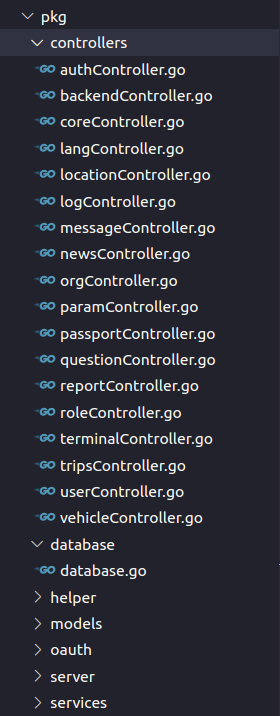
\includegraphics[scale=0.5]{v1_structure.png}
\caption{Arrival MN эхний хувилбарын бүтэц}
\end{figure}
\\
Гэсэн хэдий ч энэ нь бүтцийн буруу шийдэл болон нэг package дотор хийгдэх зүйл хэт ихсэн үндсэндээ систем monolithic болсон. Үүнээс үүдэн системийг өргөжүүлэхэд хүндрэл учран хөгжүүлэлтийн хурд удааширсан. Иймд системийн сайжруулсан хувилбарыг гаргасан ба энэхүү хувилбар нь системийн үйл ажиллагааг модульчилсан бүтцэд шилжүүлсэн. 
\\\\
\begin{figure}[H]
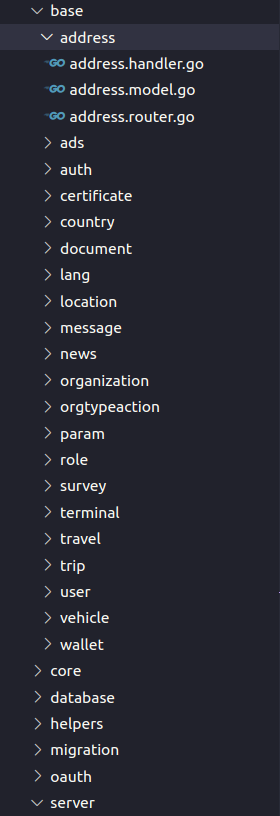
\includegraphics[scale=0.5]{v2_structure.png}
\caption{Arrival MN сайжруулсан хувилбарын бүтэц}
\end{figure}
\\ 

Модулиуд нь дараах үйл ажиллагааг гүйцэтгэдэг байна. 

\begin{table}[h]
\centering
\caption{Модулиуд}
\label{modules}
\begin{tabular}{|l|l|}
\hline
\textbf{Модулийн нэр} & \textbf{Модулийн үйл ажиллагаа}  \\ \hline
        ads           & Сурталчилгаа \\ \hline
        auth          & Бүртгүүлэх, нэвтрэх зэрэг баталгаажуулалт       \\ \hline
        country       & Улсын мэдээллэл \\ \hline
        document      & Бичиг баримт \\ \hline
        lang          & Хэлний сонголт, орчуулга \\ \hline
        location      & Байршил \\ \hline
        message       & Мессеж \\ \hline
        news          & Мэдээ \\ \hline
        organization  & Байгууллага \\ \hline
        orgtypeaction & Байгууллагын эрх \\ \hline
        param         & Параметрүүд \\ \hline
        role          & Эрх \\ \hline
        survey        & Асуумж \\ \hline
        travel        & Нислэгийн дугаарууд \\ \hline
        trip          & Хилээр нэвтэрсэн мэдээлэл \\ \hline
        user          & Хэрэглэгч \\ \hline
\end{tabular}
\end{table}


\section{Хэрэгжүүлэлтийн дэлгэрэнгүй} 

Системийн үндсэн функц нь дараах функц байх ба тодорхой өгөгдлийг олон дахин дуудаж ажиллагааг удаашруулахгүйн тулд компайль хийхэд эхэнд нь дуудан хадгалсан болно.
\\ 
\begin{lstlisting}[language=Go, caption=Үндсэн функц, frame=single]
package main

import (
	"fmt"
	"os"
	"arrival-mn-v2/pkg/database"
	"arrival-mn-v2/pkg/helpers"
	"arrival-mn-v2/pkg/helpers/logger"
	"arrival-mn-v2/pkg/migration"
	"arrival-mn-v2/pkg/oauth"
	"arrival-mn-v2/pkg/server"

	"github.com/joho/godotenv"
)

func main() {
	cmds := os.Args[1:]
	if err := godotenv.Load(".env"); err != nil {
		fmt.Println("Can't find env file")
	}

	database.Init()
	if helpers.StringInArr("--migrate", cmds) {
		migration.Run()
	}

	oauth.Init()
	logger.Init()
	server.Init()
}

\end{lstlisting}
Дээрх функцийн хувьд database-д холбогдох, oauth буюу token үүсгэх Manager, log бичих job ажиллуулж байгаа бөгөөд эдгээр нь модуль бүр ашиглах дундын нөөцүүд юм. Харин server.Init нь Go Fiber фреймворкийг ажиллуулж байгаа бөгөөд модуль бүрийн router-үүдийг дуудаж байгаа. 
\\
\begin{lstlisting}[language=Go, caption=Go Fiber эхлүүлэх, frame=single]
package server

import (
	"log"
	"os"

	"github.com/gofiber/fiber/v2"
	"github.com/gofiber/fiber/v2/middleware/cors"
	"github.com/gofiber/fiber/v2/middleware/logger"
	"github.com/gofiber/fiber/v2/middleware/recover"
	"github.com/gofiber/fiber/v2/middleware/requestid"
)

func Init() {
	app := fiber.New()
-	app.Use(requestid.New())
	app.Use(cors.New(cors.Config{
		AllowOrigins:     "*",
		AllowHeaders:     "Authorization, Content-type, Accept",
		AllowMethods:     "GET,POST,PUT,DELETE,PATCH",
		AllowCredentials: true,
	}))
	app.Use(recover.New())
	app.Use(logger.New())

	InitRoutes(app)

	log.Fatal(app.Listen(os.Getenv("PORT")))
}


func InitRoutes(app *fiber.App) {
	app.Use(core.RequestMiddleware)
	auth.SetRoutes(app)
	user.SetRoutes(app)
	role.SetRoutes(app)
	document.SetRoutes(app)
	organization.SetRoutes(app)
	terminal.SetRoutes(app)
	location.SetRoutes(app)
	vehicle.SetRoutes(app)
	country.SetRoutes(app)
	lang.SetRoutes(app)
	news.SetRoutes(app)
	orgtypeaction.SetRoutes(app)
	wallet.SetRoutes(app)
	survey.SetRoutes(app)
	trip.SetRoutes(app)
	address.SetRoutes(app)
	certificate.SetRoutes(app)
	travel.SetRoutes(app)
	ads.SetRoutes(app)
	param.SetRoutes(app)
}

\end{lstlisting}

\section{Хүсэлт боловсруулах} 

Модулийн SetRoutes нь тухайн модуль ямар замаар ирсэн хүсэлтийг хэрхэн боловсруулах тухай тодорхойлох ба аль хүсэлт нь баталгаажуулалт шаардахыг тодорхойлно. 

\\
\begin{lstlisting}[language=Go, caption=Модулийн Route хэсэг, frame=single]
package survey

import (
	"arrival-mn-v2/pkg/oauth"
	"github.com/gofiber/fiber/v2"
)

func SetRoutes(app *fiber.App) {
	var question QuestionHandler
	var group QuestionGroupHandler
	var choice QuestionChoiceHandler
	q := app.Group("question", oauth.TokenMiddleware)
	q.Get("", question.List)
	q.Post("", question.Save)
	q.Put("", question.Update)
	q.Delete("", question.Delete)

	q.Post("/save_answer", question.SaveAnswer)
	q.Get("/is_button", question.IsButton)

	g := app.Group("question/group", oauth.TokenMiddleware)
	g.Get("", group.ListGroup)
	g.Post("", group.SaveGroup)
	g.Put("", group.UpdateGroup)
	g.Delete("", group.DeleteGroup)

	c := app.Group("question/choice", oauth.TokenMiddleware)
	c.Get("", choice.List)
	c.Post("", choice.Create)
	c.Put("", choice.Update)
	c.Delete("", choice.Delete)

}

\end{lstlisting}

Router функц дотор тухайн хүсэлтэд харгалзан ямар функц дуудахыг зааж өгж байна. Тэгвэл тэдгээр функцууд нь Handler дээрх функцуудийг дуудна. Handler дээрх функцууд нь хүсэлтийн JSON хэлбэрийг модел болгон буулгах ба хүсэлтийг хэрхэн боловсруулахыг шийдвэрлэх үндсэн хэсэг болж ажиллана. Доорх жишээнд харуулсан BeforeSave нь hook үйлдэл бөгөөд өгөгдлийн санд ямар нэг үйлдэл хийхийн өмнө эсвэл дараа тухайн моделд ямар өөрчлөлт оруулахыг тусгадаг GORM-ийн функцуудын нэг юм. Ингэснээр нэг үйлдлийг олон дахин хийхээс зайлсхийж арчилгааг илүү хялбар болгодог. 

\begin{lstlisting}[language=Go, caption=Модулийн Handler, frame=single]
package survey

import (
	"arrival-mn-v2/pkg/core"
	"arrival-mn-v2/pkg/oauth"

	"github.com/gofiber/fiber/v2"
)

type QuestionHandler struct{}

func (*QuestionHandler) List(c *fiber.Ctx) error {
	var (
		res interface{}
		err error
	)

	if res, err = List(c); err != nil {
		return core.Resolve(500, c, core.Response(err.Error()))
	}
	return core.Resolve(200, c, core.Response("success", res))
}

func (*QuestionHandler) Save(c *fiber.Ctx) error {
	req := new(Question)
	if err := c.BodyParser(req); err != nil {
		return core.Resolve(400, c, core.Response(err.Error()))
	}

	if err := req.Save(); err != nil {
		return core.Resolve(500, c, core.Response(err.Error()))
	}
	return core.Resolve(200, c, core.Response())
}

func (*QuestionHandler) Update(c *fiber.Ctx) error {
	req := new(Question)
	if err := c.BodyParser(req); err != nil {
		return core.Resolve(400, c, core.Response(err.Error()))
	}

	if err := req.Update(); err != nil {
		return core.Resolve(500, c, core.Response(err.Error()))
	}
	return core.Resolve(200, c, core.Response())
}

func (*QuestionHandler) Delete(c *fiber.Ctx) error {
	req := new(Question)
	if err := c.BodyParser(req); err != nil {
		return core.Resolve(400, c, core.Response(err.Error()))
	}
	req.DeletedBy = oauth.GetSessionUserId(c)
	if err := req.Delete(); err != nil {
		return core.Resolve(500, c, core.Response(err.Error()))
	}
	return core.Resolve(200, c, core.Response())
}
\end{lstlisting}

Model дээрх функцууд нь тухайн модель болон өгөгдлийн сантай харьцах үйлдлүүдийг хийх ба үүсгэх, засах зэрэг тогтсон нэг үйлдлийг л хийдэг байна. 

\begin{lstlisting}[language=Go, caption=Модулийн Model, frame=single]
package survey

import (
	"arrival-mn-v2/pkg/base/lang"
	"arrival-mn-v2/pkg/database"
	"arrival-mn-v2/pkg/helpers"
	"arrival-mn-v2/pkg/helpers/convertor"
	"arrival-mn-v2/pkg/helpers/data"

	"github.com/gofiber/fiber/v2"
	"gorm.io/gorm"
)

type Question struct {
	Id         uint                   `json:"id" gorm:"primaryKey"`
	Type       string                 `json:"type"`
	GroupId    uint                   `json:"group_id"`
	Status     string                 `json:"-" gorm:"type:varchar(1);default:'A'"`
	Choices    []QuestionChoice       `json:"choices"`
	Answer     Answer                 `json:"answer"`
	KeyId      int                    `json:"key_id"`
	LangKey    lang.Key               `json:"lang_key" gorm:"foreignKey:KeyId"`
	IsMust     string                 `json:"is_must" gorm:"type:varchar(1);default:'N'"`
	Text       string                 `json:"text" gorm:"-"`
	Translated []lang.ResTranslations `json:"translated,omitempty" gorm:"-"`
	Ord        int                    `json:"ord" gorm:"default:0"`
	Validation string                 `json:"validation" gorm:"type:varchar(20)"`
	CreatedAt  data.LocalTime         `json:"created_date" gorm:"autoCreateTime"`
	CreatedBy  uint                   `json:"created_by,omitempty"`
	UpdatedAt  data.LocalTime         `json:"updated_date" gorm:"autoUpdateTime"`
	UpdatedBy  uint                   `json:"updated_by,omitempty"`
	DeletedAt  gorm.DeletedAt         `json:"-" gorm:"index"`
	DeletedBy  uint                   `json:"-"`
}

func (q *Question) BeforeSave(tx *gorm.DB) (err error) {
	if q.KeyId != 0 {
		return
	}
	var key lang.Key
	key, err = SaveKeyAndTranslation(q.Translated, "QUESTION")
	if err != nil {
		return err
	}
	q.LangKey = key
	q.KeyId = int(key.Id)
	return
}

func List(c *fiber.Ctx) (res []Question, err error) {
	db := database.DBconn
	groupId := convertor.StringToInt(c.Query("group_id"))
	key := c.Query("key", "DECLARATION")

	tx := db.Debug().Table(helpers.GetTableName("question")+" as question").
		Joins("INNER JOIN "+helpers.GetTableName("question_group")+" as qg ON qg.id = question.group_id").
		Where("group_id = COALESCE(nullif(?, 0), group_id)", groupId).Where("question.status = 'A'").
		Where("qg.key = ?", key)

	err = tx.Preload("LangKey").Preload("Choices").Preload("Choices.LangKey").Order("ord").Order("id").Find(&res).Error
	return
}

func (q *Question) Save() (err error) {
	db := database.DBconn
	if err = db.Create(&q).Error; err != nil {
		return
	}
	return nil
}

func (q *Question) Update() (err error) {
	db := database.DBconn
	if err = db.Model(&Question{}).Where("id = ?", q.Id).Updates(q).Error; err != nil {
		return
	}
	for _, choice := range q.Choices {
		choice.QuestionId = q.Id
		if err = choice.Create(); err != nil {
			return
		}
	}
	return nil
}

func (q *Question) Delete() (err error) {
	db := database.DBconn
	err = db.Debug().Model(&q).Update("status", "I").Error
	return
}
\end{lstlisting}

Ийнхүү router, handler, model-оос бүрдэх модуль нь харгалзах хүсэлтүүдийг боловсруулдаг. Энд жишээ болгон энгийн модулийн хэрэгжүүлэлтийг оруулсан ба тухайн хүсэлтийг боловсруулах нь төвөгтэй байх тусам handler дээрх ашиглах model-ийн функцууд олон болох юм. 

\section{Хянах системийн front-end хэсэг}

Системийн үндсэн хуудсууд нь дараах хуудсууд байх ба хэрэглэгчдэд хялбар байх үүднээс үндсэн систем, хянах систем гэсэн хоёр модульд хуваасан болно.

\\ 
\begin{lstlisting}[language=HTML, caption=Үндсэн хуудас, frame=single]
<template>
  <Loader />
  <router-view></router-view>
</template>
<script lang="ts">
import { defineComponent } from "vue";
import { mapMutations, mapActions } from "vuex";
import storage from "./helpers/storage.helper";
import Loader from "./components/Loader.vue";

export default defineComponent({
  components: { Loader },
  mounted() {
    this.loadLang();
    this.loadTranslation();
    this.setUser(storage.get("user"));
    this.setToken(storage.get("token"));
    this.setSelectedPath(storage.get("path"));
    this.setOrganizations(storage.get("organizations"));
    this.setSelectedOrganization(storage.get("selectedOrganization"));
    this.getRole(storage.get("role"));
    this.setSelectedLanguage(storage.get("selectedLanguage"));
  },
  methods: {
    ...mapMutations([
      "setUser",
      "setToken",
      "setSelectedPath",
      "setSelectedOrganization",
      "setOrganizations",
      "setLanguages",
      "setSelectedLanguage",
    ]),
    ...mapActions(["getRole"]),

    async loadTranslation() {
      const translations = await this.$api("/translation?", "get");
      storage.set("translations", translations.result.items);
    },
    async loadLang() {
      const languages = await this.$api("/language", "get");
      this.setLanguages(languages.result.items);
      if (!storage.get("selectedLanguage")) {
        this.setSelectedLanguage(languages.result.items[0]);
      }
    },
  },
});
</script>

\end{lstlisting}
Дээрх хуудсын хувьд үндсэн хуудас бөгөөд системийн хуудсуудыг харахын тулд router нэрийг ашиглан дуудах бөгөөд веб хөтөчийн Local storage-ыг ашиглан хадлаглсан мэдээллүүдийг авч хүсэлтийн боловсруулан UI-ийг зурж байгаа юм.
\\
\begin{lstlisting}[language=java, caption=Vue application эхлүүлэх үндсэн функц, frame=single]
import { createApp } from "vue";
import App from "./App.vue";
import "./assets/index.css";
import routes from "./routes";
import store from "./store";

import { Store } from "vuex";
import { Router } from "vue-router";
import apiPlugin from "./plugins/api.plugin";
import noticePlugin from "./plugins/notice.plugin";
import permissionPlugin from "./plugins/permission.plugin";
import loaderPlugin from "./plugins/loader.plugin";
import commonPlugin from "./plugins/common.plugin";
import i18nPlugin from "./plugins/i18n.plugin";

import ElementPlus from "element-plus";
import mn from "element-plus/es/locale/lang/mn";
import "element-plus/dist/index.css";
import Page from "./components/Page.vue";
import Table from "./components/Table.vue";
import Vue3DraggableResizable from 'vue3-ts-draggable-resizable';

declare module "vue" {
  interface ComponentCustomProperties {
    $router: Router;

    $api: Function;

    $apifile: Function;

    $store: Store<any>;

    $notice: Function;

    $translate: Function;

    $loader: Function;

    $permission: Function;

    $writeExcel: Function;

    $calculateModalWidth: Function;
    $amountFormatter: Function;
    $amountParser: Function;
    $calculateModalTop: Function;
    $nameReturner: Function;
  }
}

const app = createApp(App);
/* Плагинууд */
app.use(ElementPlus, { locale: mn });
app.use(store);
app.use(routes);
app.use(apiPlugin, store);
app.use(noticePlugin, store);
app.use(permissionPlugin, store);
app.use(loaderPlugin, store);
app.use(commonPlugin);
app.use(i18nPlugin, store);
app.component('vue3-draggable-resizable', Vue3DraggableResizable);
app.component("Page", Page);
app.component("DataTable", Table);

app.mount("#app");

\end{lstlisting}
Дээрхи функц нь бусад газар бичигдэн экспорт хийгдсэн функцууд болон component-үүдийг глобалчилах буюу хүссэн газраа импортлох шаардлагагүйгээр функцын эсвэл component-ийн нэрээр дуудаж ашиглах боломжтой болгож байгаа юм.

\\ 
\begin{lstlisting}[language=java, caption=API дуудах үндсэн глобар функц, frame=single]
import axios from "axios";

/**
 * Промайс гүйцэтгэгч
 * @param promise Промайс обект
 * @returns Биелсэн эсвэл Цуцалсан обьект
 */
const resolver = (promise: Promise<any>): any => {
  return promise
    .then((resolve) => {
      return [null, resolve];
    })
    .catch((reject) => {
      return [reject, null];
    });
};

/**
 * хүсэлт илгээгч
 * @param url хүсэлт илгээх эндпойнт
 * @param headers хүсэлтийн толгой хэсэг
 * @param method хүсэлтийн method
 * @param data хүсэлтийн бие
 * @returns Промайс обьект
 */

const fetcher = (url: string, headers: any, method: any, data: any) => {
  return new Promise((resolve, reject) => {
    axios
      .request({
        method: method,
        url: url,
        data: data,
        headers: headers,
      })
      .then((httpResponse) => {
        resolve(httpResponse);
      })
      .catch((err) => {
        reject(err);
      });
  });
};

export default { resolver, fetcher };

\end{lstlisting}

\\ 
\begin{lstlisting}[language=java, caption=API дуудсан фунцаас ирсэн response дээр боловсруулалт хийх функц, frame=single]
import { App } from "vue";
import { Store } from "vuex";
import router from "../routes";
import client from "../helpers/api.helper";
import { URL_MAIN, URL_FILE } from "../helpers/config.helper";

export default {
  install: (app: App, store: Store<any>) => {
    app.config.globalProperties.$apifile = async (path: String, data: FormData) => {
      let message = "";
      const notice = app.config.globalProperties.$notice;
      try {
        const url = URL_FILE + path;
        const headers: any = {};
        if (path == "/remove") {
          headers["Authorization"] = `Bearer ${store.getters.token}`;
        } else {
          headers["Authorization"] = `Bearer ${store.getters.token}`;
          headers["Content-Type"] = `multipart/form-data`;
        }
        const [err, res] = await client.resolver(client.fetcher(url, headers, "post", data));
        if (err) {
          if (err.response && err.response.status && err.response.status === 401) {
            store.commit("setUser", null);
            router.push("/login");
            message = "Холболт салсан байна.";
          } else {
            message = "Интернэт холболтоо шалгана уу: " + err.message;
          }

          notice(message, "error", true, 5000);
          return null;
        }

        if (res.code === 401) {
          store.commit("setUser", null);
          router.push("/login");
          return null;
        }

        if (res.code !== 200) {
          message = res.message;
          notice(message, "error", true, 5000);
          return null;
        }

        return res.result;
      } catch (error: any) {
        message = "Алдаа: ";
        if (error.message) message += error.message;
        notice(message, "error", true, 5000);
        return null;
      }
    };

    app.config.globalProperties.$api = async (url: string, method: any, data = {}) => {
      let message = "";
      const notice = app.config.globalProperties.$notice;

      try {
        const requestUrl = URL_MAIN + url;
        const headers: any = {};
        headers["Authorization"] = `Bearer ${store.getters.token}`;

        const [err, res] = await client.resolver(client.fetcher(requestUrl, headers, method, data));
        if (err) {
          if (err.response && err.response.status && err.response.status === 401) {
            store.commit("logout");
            message = "Холболт салсан байна.";
          } else {
            message = err.response.data.message;
          }

          notice(message, "error", true, 5000);
          return null;
        }

        if (res.status === 401) {
          store.commit("logout");
          notice(res.message, "error", true, 5000);
          return null;
        }

        if (res.status === 201) {
          return "201";
        }

        return res.data;
      } catch (error: any) {
        message = "Алдаа: ";
        if (error.message) message += error.message;
        notice(message, "error", true, 5000);
        return null;
      }
    };
  },
};

\end{lstlisting}

Дээрхи функцууд нь api дуудах ерөнхий болон боловсруулалт хийх функцууд бөгөөд parameter-ээр орж ирсэн url, header, method, body дагуу back-end лүү хүсэлт явуулан үр дүнгээ авахад зориулагдсан болно.


\\ 
\begin{lstlisting}[language=HTML, caption=API дуудах үндсэн глобар функц, frame=single]
<template>
  <div class="w-full h-full bg-white p-4 rounded-md border border-gray-200 shadow overflow-y-auto overflow-x-hidden">
    <slot></slot>
  </div>
</template>

<script lang="ts">
import { defineComponent } from "vue";
export default defineComponent({
  name: "Page",
});
</script>
Дээрхи код нь систем дээр ашигласан vue js-ын нэг page component бөгөөд Код 5.7 дээр глобалчилагдан бүх фейж дээр ашигладаг component юм.

\end{lstlisting}

\section{Системийн UI} 

Доорхи зургууд web application-ы ерөнхий UI буюу element plus болон tailwind scc фреймворкуудыг ашиглан зурсан бөгөөд бүх кодыг оруулах боломжгүй тул бүх фейж дээр ашигласан гол код болох /Код 5.8, 5.9, 5.10/ функц, component-үүдийг дээр дурдсан болно.

\\\
\begin{figure}[H]
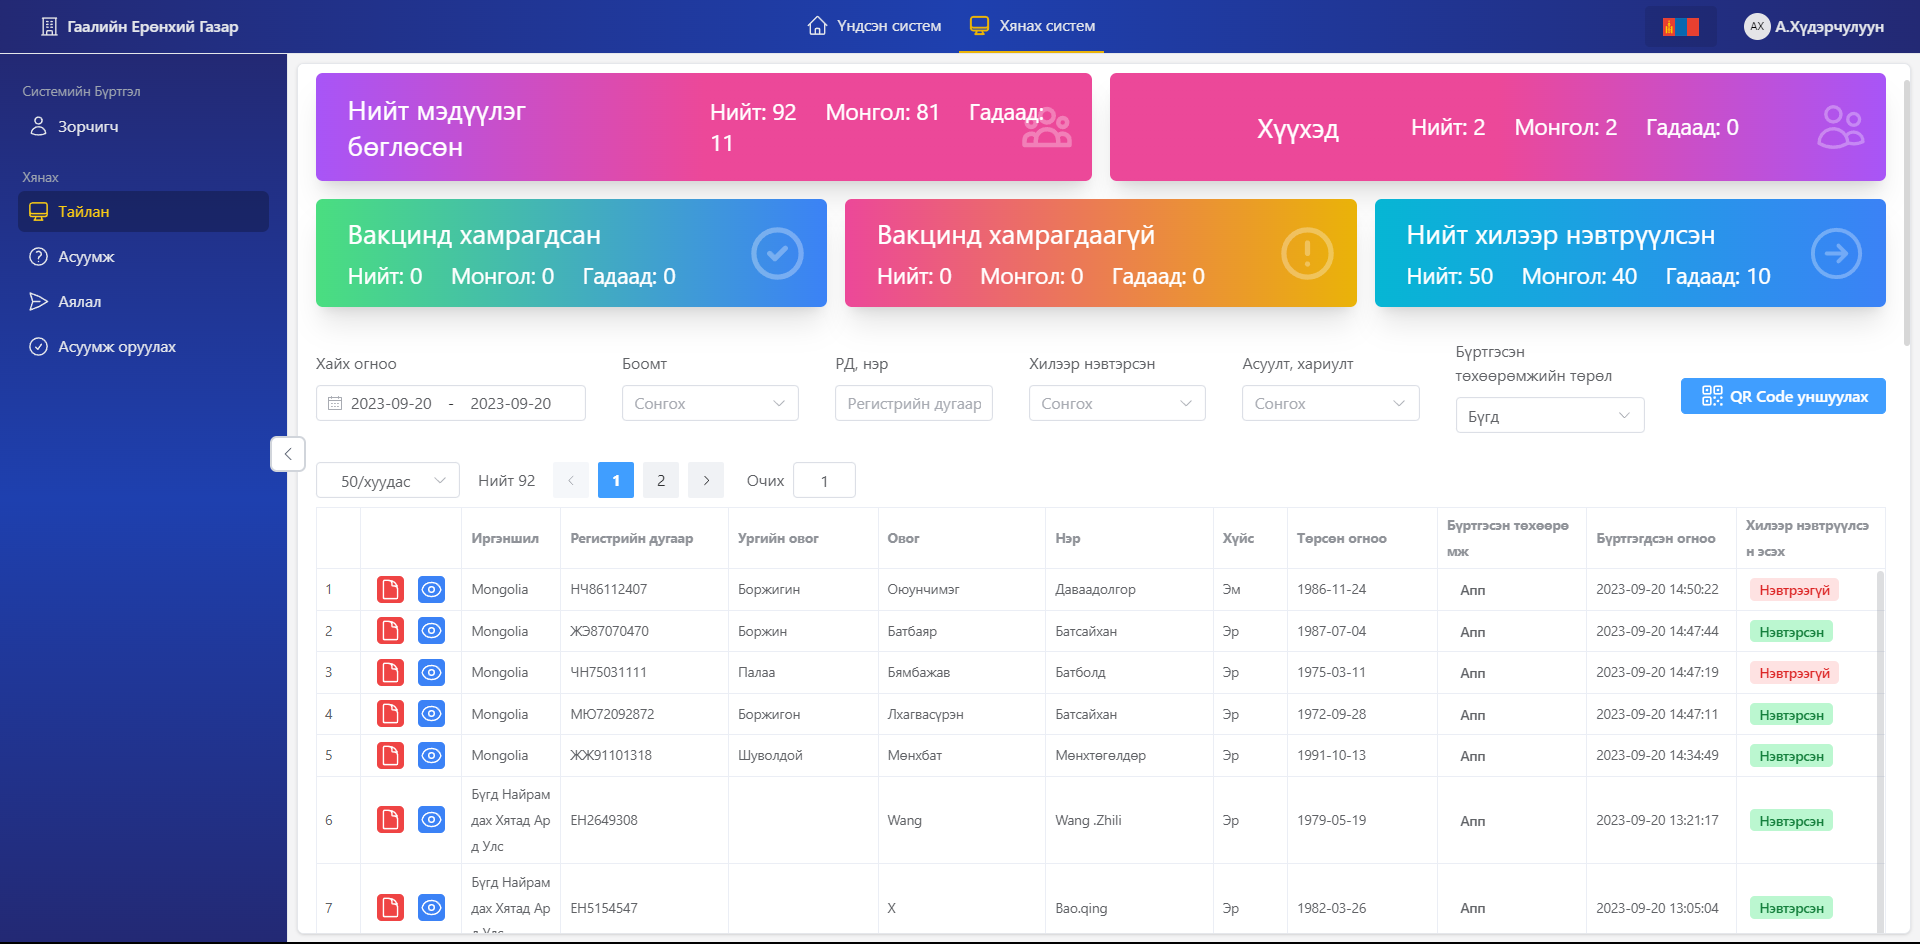
\includegraphics[scale=0.4]{report.png}
\caption{Тайлан хуудас}
\end{figure}
\\
Энэхүү хуудсаас эрүүл мэндийн асуулга бөглөсөн иргэдийн мэдээлэл, бөглөсөн асуумжийн хариулт харах боломжтойгоос гадна нийт асуумж бөглөсөн иргэдийн тоо /нийтээр, гадаад, монгол/ харах, функционал шаардлагуудын дагуу иргэдийн мэдээллийг шүүж харах, байцаагч QR уншуулж иргэний асуумжийг харах хэсгүүдийг харж болно.

\\\
\begin{figure}[H]
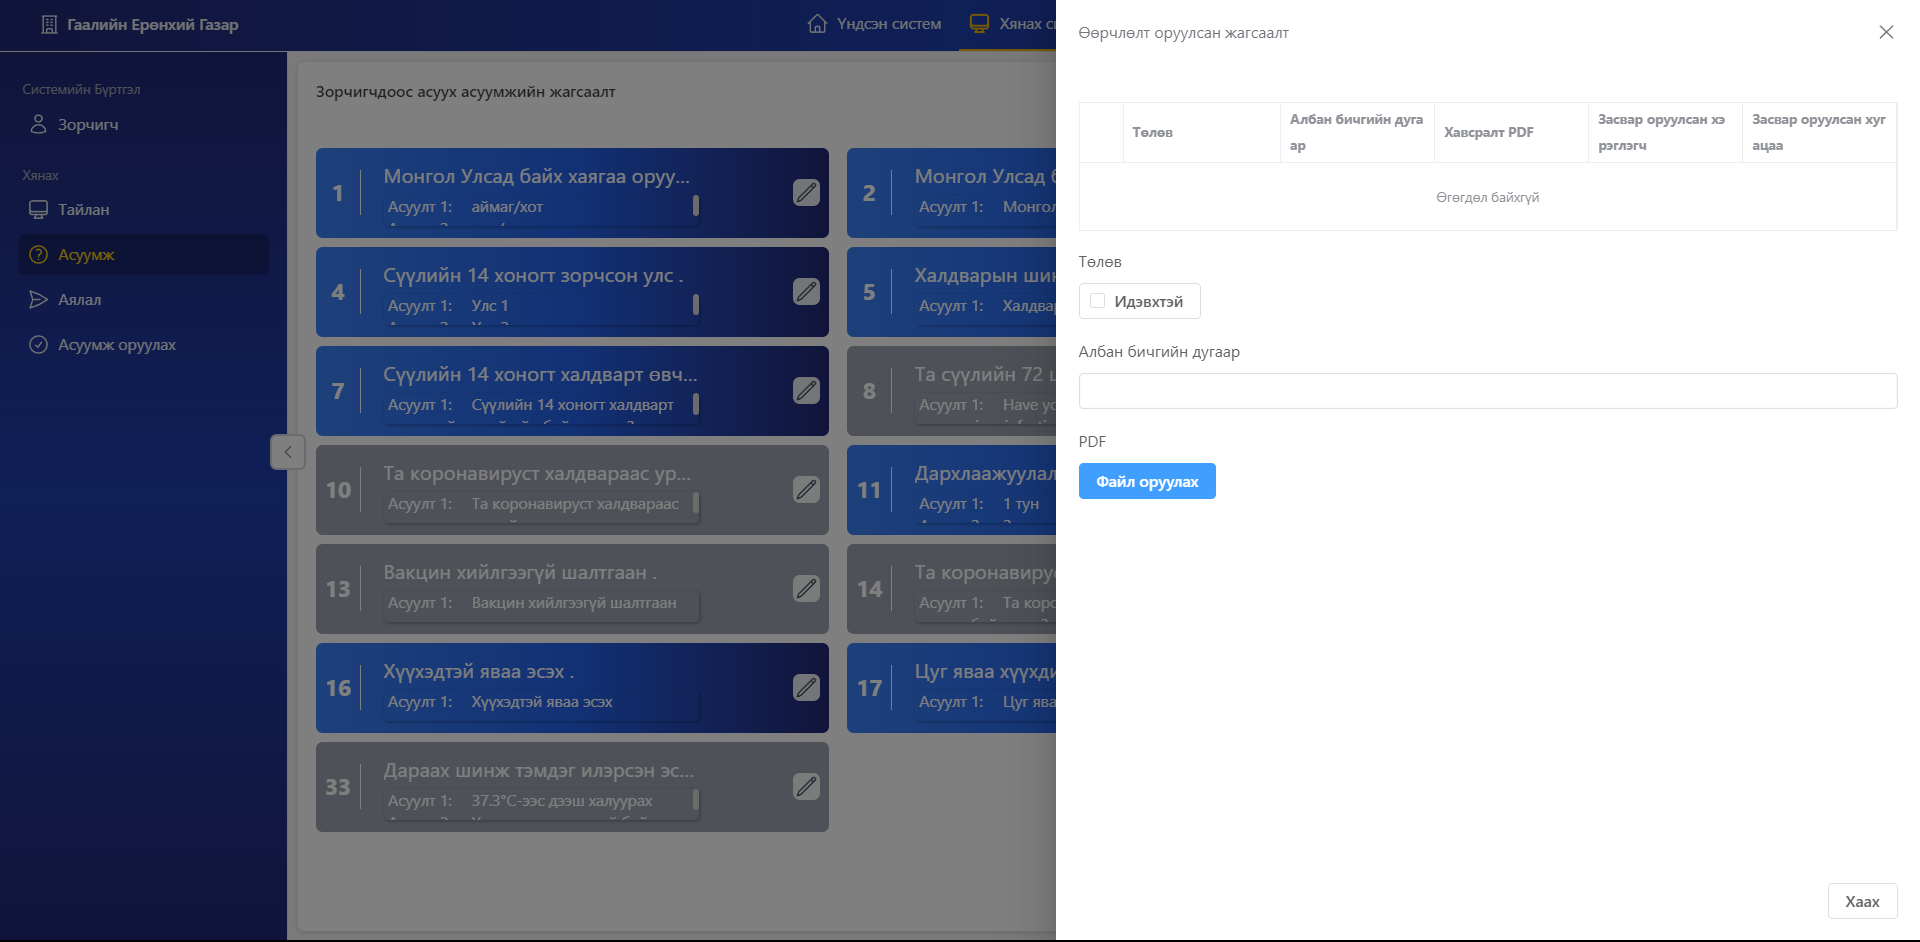
\includegraphics[scale=0.4]{questions.png}
\caption{Асуумж хуудас}
\end{figure}
\\
Дээрхи хуудас дээр хилээр нэвтрэн орж ирж буй иргэдээс асуух эрүүлж мэндийн асуумжийн жагсаалт байх ба асуумж шинээр бүртгэх, устгах, эрэмбэлэх, асуумж идвэхигүй болгох зэрэг үйлдлүүд хийх боломжтой.

\\\
\begin{figure}[H]
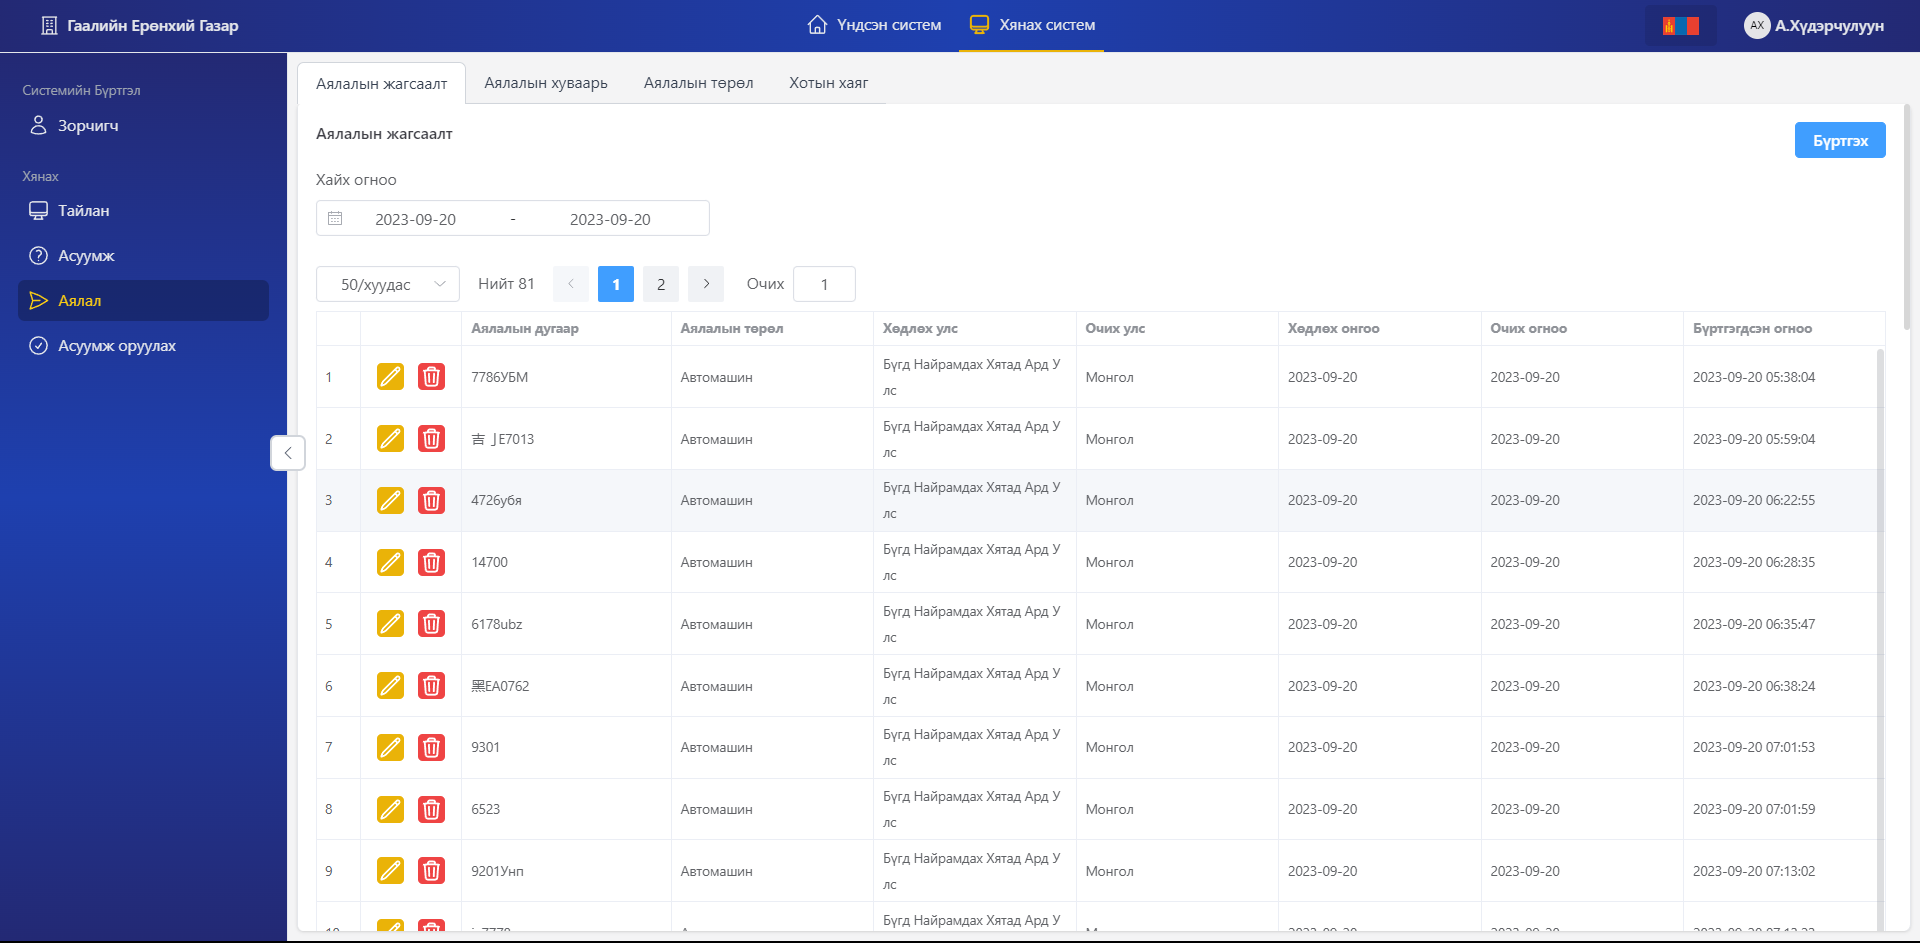
\includegraphics[scale=0.4]{travel.png}
\caption{Асуумж хуудас}
\end{figure}
\\

Дээрхи хуудсаас аялалын жагсаалт, аялалын хуваарь, аялалын төрөл, хотыг хаяг зэргийг харах боломжтой ба Use case дээр зурсаны дагуу ээлжийн ахлах ашиглах цонх юм. Аялалын жасаалт, төрөл, хуваариудыг бүртгэх, устгах засах боломжтой юм.

\\\
\begin{figure}[H]
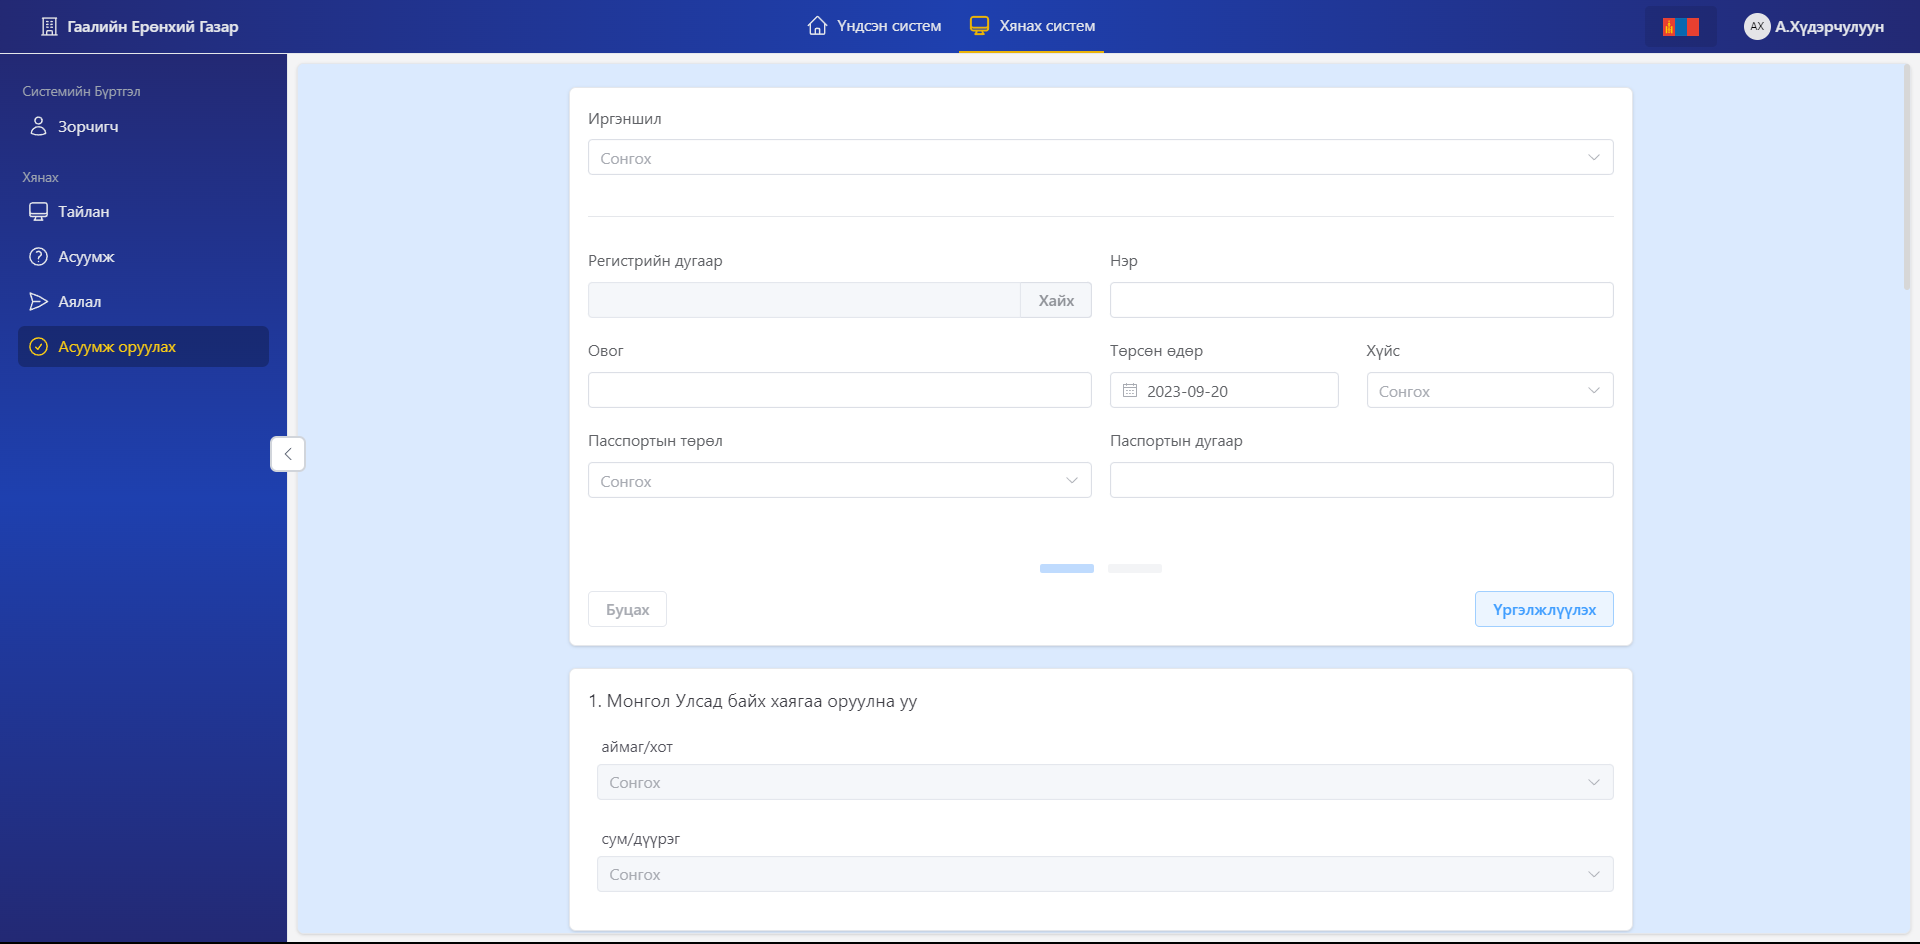
\includegraphics[scale=0.4]{enter-questions.png}
\caption{Асуумж оруулах хуудас}
\end{figure}
\\
Энэ хуудас нь эрүүл мэндийн хуудсыг ямар нэгэн байдлаас хамааран бөглөх боломжгүй иргэдийн өмнөөс байцаагч бөглөж өгөх зориулалттай ашиглах хуудас бөгөөд иргэний мэдээллийг иргэншилийн дагуу бөглөж дууссаны дараа эрүүл мэндийн асуумжийг бөглөх боломжтой болох юм.

\section{Хэрэгжүүлэлтийн дүгнэлт} 

Системийн эхний хувилбар нь бүтцийн хувьд хүндрэлтэй, зарим талаараа монолит шинжтэй байснаас үүдэн арчилахад хүндрэлтэй байснийг модульчилснаар арчилахад илүү хялбар болсон. Эндээс системийг дэд хэсгүүдэд салгах нь бүтцийн хувьд илүү зөв шийдэл гэдгийг ойлгосон. Системийг хуртай холбохын тулд хуртай холбох хэсгийг python хэлэн дээр хийхэд хэрэгжүүлэлтийн хувьд хялбар байсан хэдий ч гүйцэтгэлийн хурд удааширсан. Харин golang хэл дээр холболт хийхэд гүйцэтгэл харьцангуй сайжирсан ч хэрэгжүүлэлт нь төвөгтэй болсон. Эндээс golang нь хурдан ажиллагааны хувьд давуу талтай боловч сүүлийн үеийн хэл тул баримт бичиг, package зэрэг харьцангуй багатай хэл юм. 

